\documentclass[helvetica]{beamer}
\usetheme{Boadilla}
\input{xy}
\xyoption{all}
\usepackage{graphicx} 
\usepackage{slidesec} 
\usepackage{url}
\usepackage[framemethod=TikZ]{mdframed}
\usepackage{tikz}
\usetikzlibrary{calc,quotes,arrows.meta}
\usepackage{color}
\usepackage[normalem]{ulem}
\usepackage{verbatim}
\setbeamertemplate{itemize items}[circle]
\def\dash---{\unskip\kern.16667em---\penalty\exhyphenpenalty\hskip.16667em\ignorespaces}
\long\def\symbolfootnote[#1]#2{\begingroup%
\def\thefootnote{\fnsymbol{footnote}}\footnote[#1]{#2}\endgroup}

\title{MIMI Transport Requirements}
\author{Eric Rescorla \\\url{ekr@rtfm.com}}
\date{2022-11-10}

\begin{document}

\begin{frame}
  \titlepage
\end{frame}

\begin{frame}{Abstract Architecture}

  \vspace{.2in}
\begin{center}
  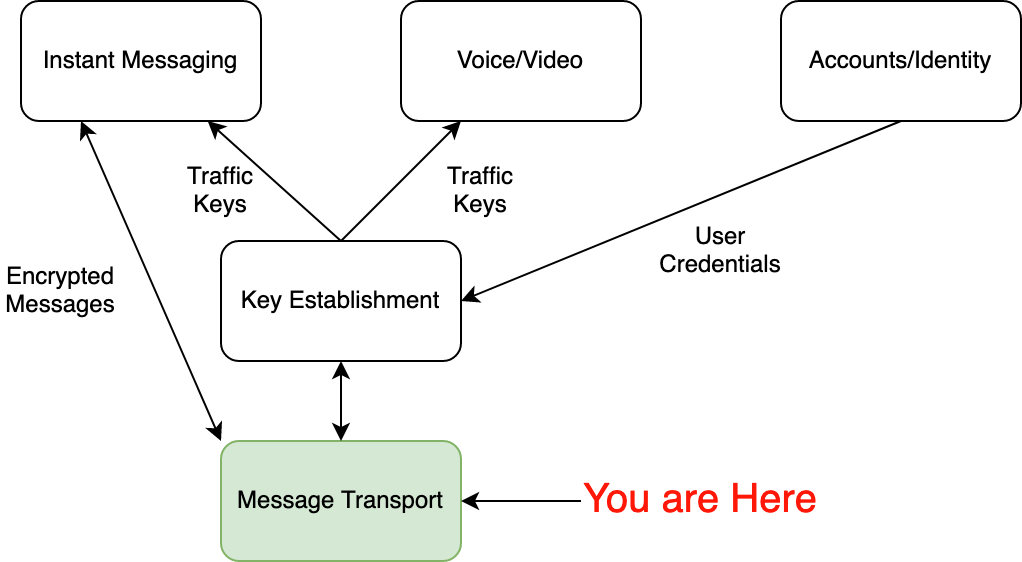
\includegraphics[width=4in]{messaging-architecture}
\end{center}
\end{frame}


\begin{frame}{Protocol Breakdown}

  \vspace{.2in}
\begin{center}
  \includegraphics[width=4in]{messaging-setting}
\end{center}
\end{frame}

\begin{frame}{Question: How much are we defining?}

  \begin{itemize}
  \item A full system obviously needs a client to-server protocol
    \begin{itemize}
    \item Message protection and content need to be E2E
    \item ... but message transport is not      
    \end{itemize}
  \item Most existing systems (XMPP, SIMPLE, etc. do it all)
  \item Is client $\longleftrightarrow$ server in scope?
  \end{itemize}  
\end{frame}


\begin{frame}{Naming and discovery}

  \begin{itemize}
  \item Two main kinds of existing identifiers
    \begin{itemize}
    \item \emph{System Specific (SSI).} e.g., ``\texttt{1.650.555.1000} on WhatsApp''
      (or maybe \texttt{mimi:16505551000@whatsapp.com})
    \item \emph{System Independent (SII):} e.g., \texttt{1.650.555.1000} or \texttt{ekr}
    \end{itemize}
  \item In general, an SII isn't enough to automatically contact someone
    \begin{itemize}
    \item You don't know what system they are on
    \item The same SII may appear on multiple systems (e.g., phone numbers on WhatsApp + iMessage)
    \end{itemize}
  \item \emph{Discovery} is the process of determining which system(s) an SII appears on
  \end{itemize}
\end{frame}

\begin{frame}{Question: Do we need to support discovery?}
  
  \begin{enumerate}
    \item Only solve for SSIs
    \item Solve for SSIs now and build discovery separately
    \item Integrate discovery and consent (SPIN, draft-rosenberg)
      \begin{itemize}
      \item These designs assume that the SII is actually an SSI in some other system
      \item What about systems that just use handles?
      \end{itemize}
  \end{enumerate}      
\end{frame}

\begin{frame}{Consent?}
  
\includegraphics[width=3in]{archer-spam}
  \begin{itemize}
  \item Alice just send messages to Bob if she has his identifier
    \begin{itemize}
    \item This is a spam vector      
    \end{itemize}
  \item Or does she need to get consent first?
    \begin{itemize}
    \item Typically this consists of sending an \emph{invite}
    \item ... Bob has to accept before seeing Alice's messages      
    \end{itemize}
  \end{itemize}
\end{frame}


\begin{frame}{KeyPackage Availability}
  \begin{itemize}
  \item Sending encrypted messages requires the KeyPackage
  \item This leaks whether the recipient exists
    \begin{itemize}
    \item Some ideas around fake KeyPackages but I don't think they work
      \end{itemize}
  \item Potential risk of KeyPackage exhaustion
  \end{itemize}
\end{frame}

\begin{frame}{Question: which modes do we support?}
  \begin{enumerate}
  \item Alice can send messages to Bob immediately    
  \item Alice can send messages to Bob but they're quarantined until Bob accepts
    \begin{itemize}
    \item Potential concerns about excess data on Bob's side      
    \end{itemize}
  \item Alice can't do anything until Bob consents
\end{enumerate}    
\end{frame}


\begin{frame}{Messages and Channels}
  \begin{itemize}
  \item (At least) three modalities
    \begin{itemize}
    \item 1-1 messages
        \item Group messages
    \item Channels/rooms
    \end{itemize}
    
  \item Some overlap between group messages and channels
  \item What about multiple group messages (or 1-1 messages) with the same membership?
    \begin{itemize}
    \item This is handled inconsistently
    \end{itemize}
  \end{itemize}
\end{frame}

\begin{frame}{Question: What models do we support?}

  \begin{enumerate}
  \item Everything's a group (this is what MLS thinks)
    \begin{itemize}
    \item Is this rich enough? What about moderation, etc.?      
    \end{itemize}
  \item Channels are fundamentally different (XMPP, Slack, etc.)
    \begin{itemize}
    \item And maybe we don't need group messages?
      \end{itemize}
  \end{enumerate}
\end{frame}

\end{document}